\documentclass[UTF8]{ctexart}
\usepackage{graphicx}
\usepackage{multirow}
\usepackage{booktabs}
\usepackage{latexsym}
\usepackage{indentfirst}
\setlength{\parindent}{2em}
\usepackage{color}
\definecolor{lbcolor}{rgb}{0.9,0.9,0.9}
\usepackage{listings}
\lstset{backgroundcolor=\color{lbcolor}}
\lstset{keywordstyle=\color[rgb]{0,0,1}}
\lstset{commentstyle=\color[rgb]{0.133,0.545,0.133}}
\lstset{stringstyle=\color[rgb]{0.627,0.126,0.941}}
\lstset{language=Matlab}
\lstset{numbers=left}
\lstset{breaklines=true}
\author{何舜成}
\date{2012011515}
\title{Image Processing Exercise 4}
\begin{document}
\maketitle
\section{问题描述}
有如下图像,请实现直方图均衡化增强该图像的对比度。\par
\begin{figure}[htbp]
\centerline{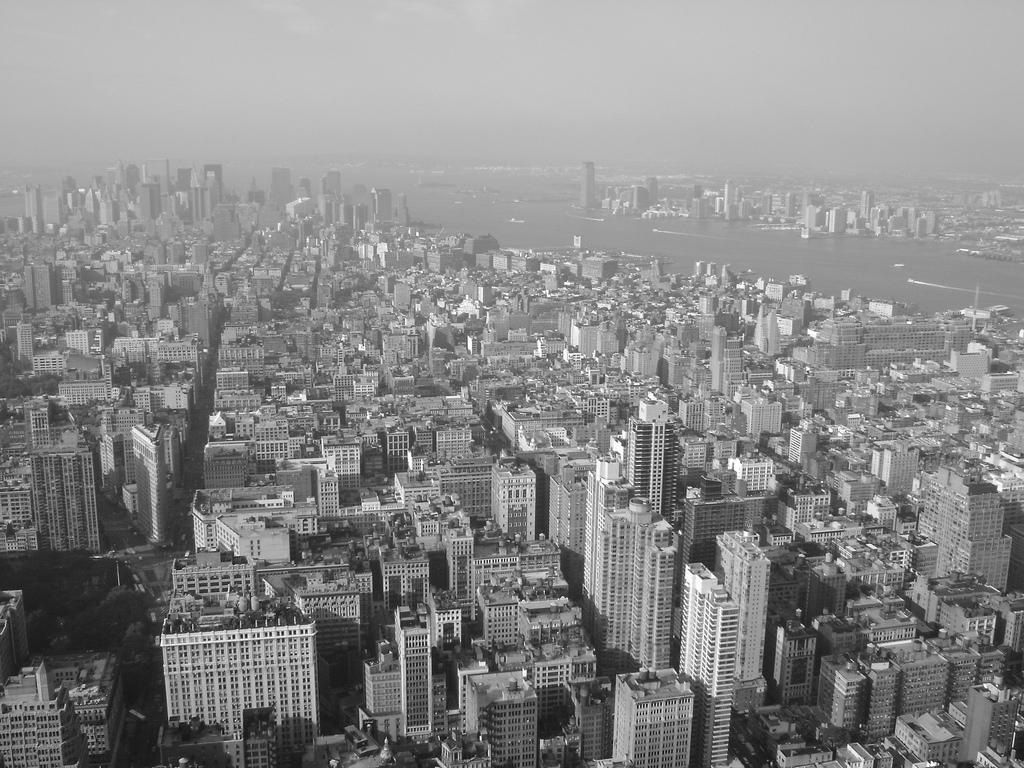
\includegraphics[width=3.5in]{hw4.jpg}}
\caption[]{original image}
\end{figure}
\section{问题解答}
直方图反映了图像不同灰度值在不同取值上的概率分布,直方图越均匀,图片对比度强,直方图越集中,对比度越差。实际操作中,应先计算图片的直方图,然后计算累积概率分布,根据图2做直方图校正。\par
\begin{figure}[htbp]
\centerline{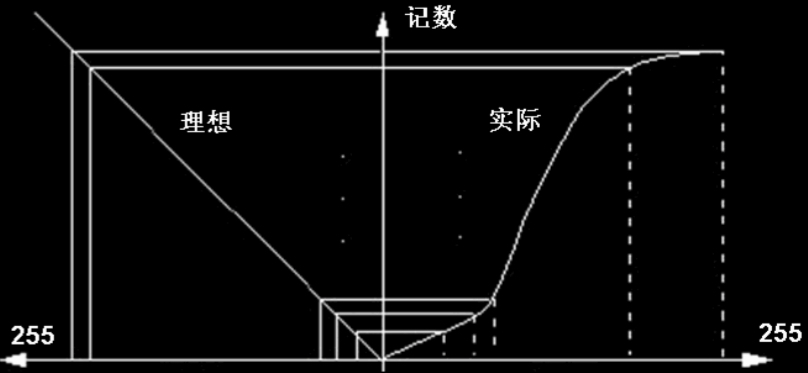
\includegraphics[width=4.5in]{prin.jpg}}
\caption[]{algorithm}
\end{figure}\par
直方图均衡化之后如图3,相比图1,图片的对比度得到明显增强。\par
\begin{figure}[htbp]
\centerline{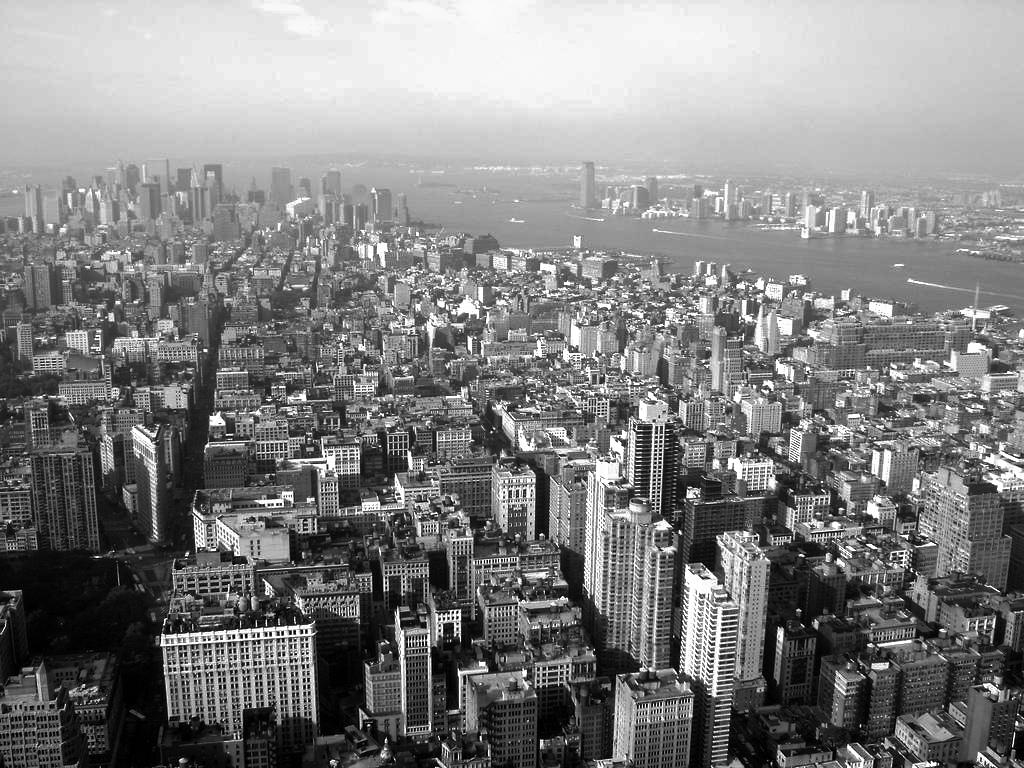
\includegraphics[width=3.5in]{rect.jpg}}
\caption[]{rectified image}
\end{figure}\par
原图与校正图的直方图如图4、图5,可以看到原图的直方图较为集中,校正图的直方图较为平均,由于量化误差的存在,校正后的直方图不是完全平均的。\par
\begin{figure}[htbp]
\centerline{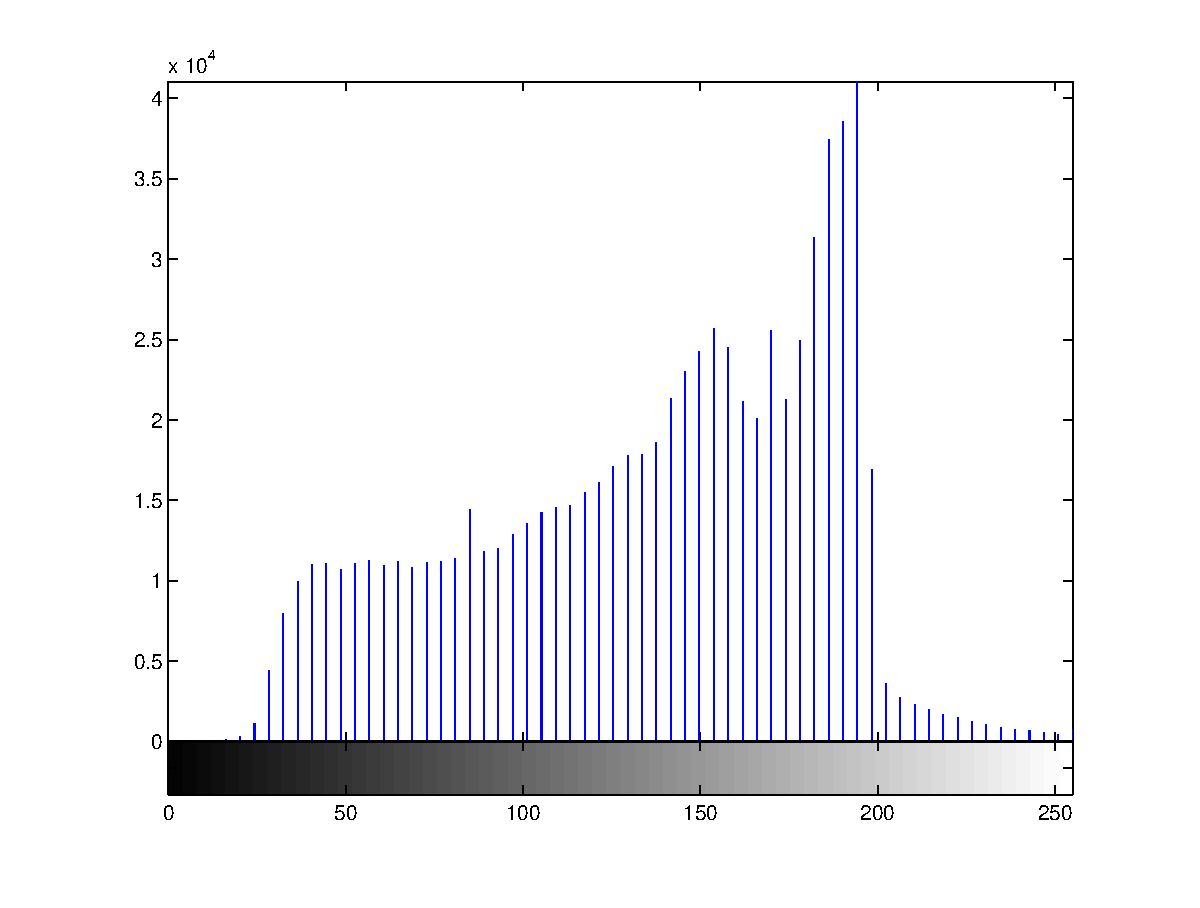
\includegraphics[width=3in]{raw.eps}}
\caption[]{histogram of original image}
\end{figure}\par
\begin{figure}[htbp]
\centerline{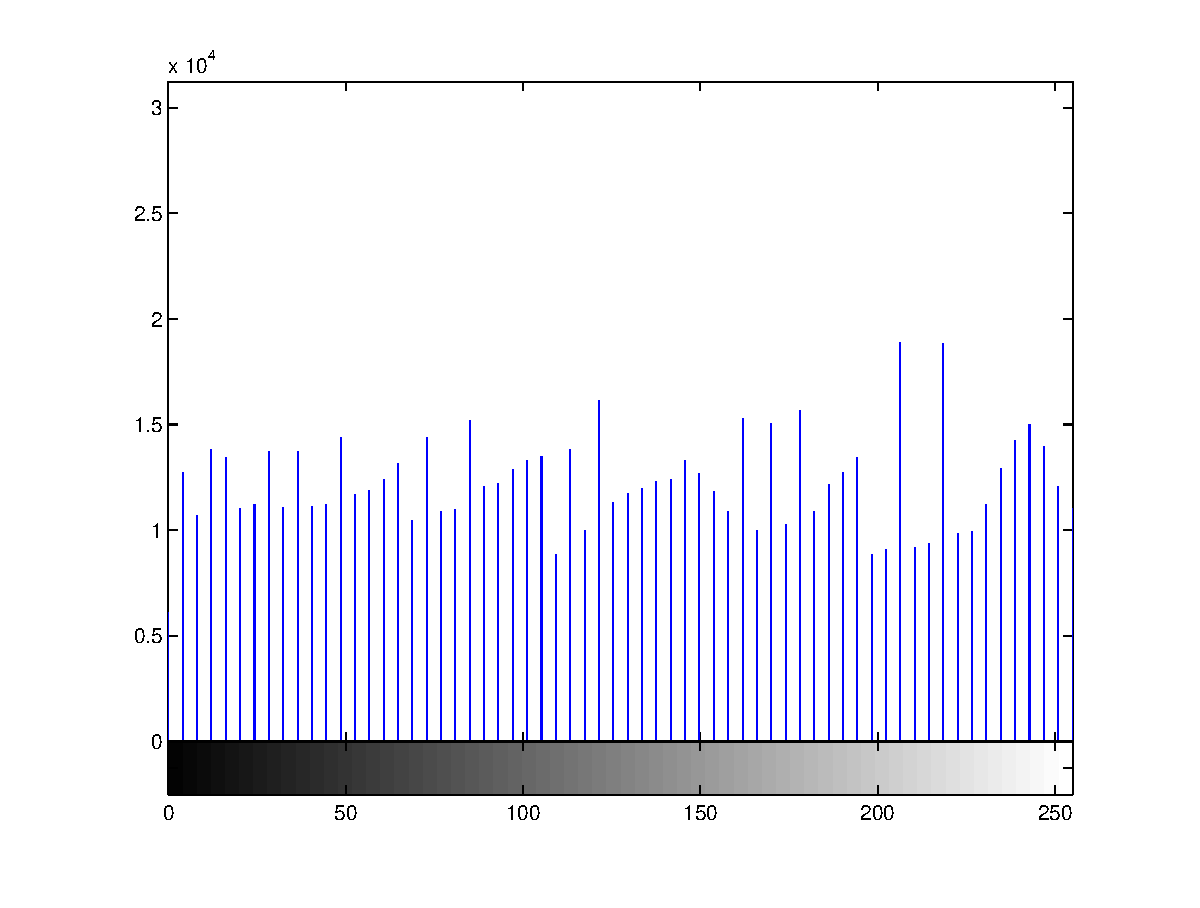
\includegraphics[width=3in]{rect.eps}}
\caption[]{histogram of rectified image}
\end{figure}\par
源码为Matlab,运行环境为Matlab R2013a,Mac OS X版。
\end{document}